\chapter{Equations of Motion}

Consider a single, unconstrained finite element~$i$ with~$n$ degrees of freedom.
Its configuration at time~$t$ will be described by the displacement vector~$\boldsymbol{u}_i(t) \in \mathbb{R}^n$ containing all positions and rotation angles of the nodes.
The equation of motion for the kind of elements we're concerned with takes the form

\begin{equation}
\boldsymbol{M}_i\,\ddot{\boldsymbol{u}}_i + \boldsymbol{q}_i(\boldsymbol{u}_i,\,\dot{\boldsymbol{u}}_i) = \boldsymbol{p}_i(t).\label{eq:local-equation-of-motion}
\end{equation}

This is a nonlinear ordinary differential equation of second order for the displacements.
$\boldsymbol{M}_i \in \mathbb{R}^{n \times n}$ is called the element's mass matrix,~$\boldsymbol{q}_i \in \mathbb{R}^n$ is the vector of internal forces depending on the displacements and their associated velocity (e.g. elastic forces, damping forces, \ldots) and~$\boldsymbol{p}_i \in \mathbb{R}^n$ is the vector of externally applied loads.

Now consider a finite element system that consists of a number of such elements that are connected to each other in a certain way.
If the overall system has a total of~$N$ degrees of freedom, it's configuration can be described by the global displacement vector~$\boldsymbol{u}(t) \in \mathbb{R}^{N}$.
The local element displacements~$\boldsymbol{u}_i$ are now no longer independent but instead directly related to the global displacements of the system they are part of.
In our case these relationships can be written as

\begin{equation}
\boldsymbol{u}_i = \boldsymbol{T}_i\,\boldsymbol{u},\label{eq:kinematics-local-global}
\end{equation}

where~$\boldsymbol{T_{i}} \in \mathbb{R}^{\mathlarger{n} \times N}$ is a constant transformation matrix for the respective element.
Using the local equations of motion~(\ref{eq:local-equation-of-motion}), the kinematic relationship~(\ref{eq:kinematics-local-global}) and some analytical mechanics it can be shown \textcolor{red}{[add citation]} that the equation of motion of the overall system takes the similar form

\begin{equation}
\boldsymbol{M}\,\ddot{\boldsymbol{u}} + \boldsymbol{q}(\boldsymbol{u},\,\dot{\boldsymbol{u}}) = \boldsymbol{p}(t).
\end{equation}

where the global mass matrix $\boldsymbol{M} \in \mathbb{R}^{N \times N}$, internal forces~$\boldsymbol{q} \in \mathbb{R}^{N}$ and external forces $\boldsymbol{p} \in \mathbb{R}^{N}$ are calculated from the local element matrices as

\begin{align}
\boldsymbol{M} &= \sum_i\boldsymbol{T}_i^\mathsf{T}\, \boldsymbol{M}_i\,\boldsymbol{T}_i,\\
\boldsymbol{q} &= \sum_i\boldsymbol{T}_i^\mathsf{T} \boldsymbol{q}_i(\boldsymbol{T}_i\,\boldsymbol{u},\,\boldsymbol{T}_i\,\dot{\boldsymbol{u}}),\\
\boldsymbol{p} &= \sum_i\boldsymbol{T}_i^\mathsf{T}\,\boldsymbol{p}_i.
\end{align}

In practice, because of the way the element displacements are related to the overall displacements, the transformation matrices~$\boldsymbol{T}_i$ only contain ones and zeros, effectively describing a selection of entries.
Therefore it is not actually necessary to carry out all the matrix multiplications occurring above.
Instead, the entries of the local matrices can be directly added to the corresponding entries of the global matrices.

In order to solve the equations of motion for equilibrium we're later going to need the derivative of the internal forces with respect to the displacements, which is called the tangent stiffness matrix~$\boldsymbol{K} \in \mathbb{R}^{N \times N}$ of the system,

\begin{equation}
\boldsymbol{K}(\boldsymbol{u}) = \frac{\partial \boldsymbol{q}}{\partial \boldsymbol{u}}
\end{equation}

It can be calculated from the element's local tangent stiffness matrices~$\boldsymbol{K}_i = \frac{\partial \boldsymbol{q}_i}{\partial \boldsymbol{u}_i}$ like this,

\begin{align*}
\boldsymbol{K}(\boldsymbol{u}) &= \frac{\partial \boldsymbol{q}}{\partial \boldsymbol{u}} = \sum_i\boldsymbol{T}_i^\mathsf{T} \frac{\partial \boldsymbol{q}_i}{\partial \boldsymbol{u}} = \sum_i\boldsymbol{T}_i^\mathsf{T} \frac{\partial \boldsymbol{q}_i}{\partial \boldsymbol{u}_i} \frac{\partial \boldsymbol{u}_i}{\partial \boldsymbol{u}} = \sum_i\boldsymbol{T}_i^\mathsf{T} \frac{\partial \boldsymbol{q}_i}{\partial \boldsymbol{u}_i} \boldsymbol{T}_i\\
&= \sum_i\boldsymbol{T}_i^\mathsf{T} \boldsymbol{K}_i \boldsymbol{T}_i.
\end{align*}

For now this is all we have to know about the equations of motion of the finite element system.
What's going to be needed next are the local equations of motion for the different element types.
Those are going to be derived in the next sections.

\newpage
\section{Mass Element}

The point mass is the most simple element.
Figure~\ref{fig:elements:point-mass} shows its definition: A mass~$m$ is placed in a cartesian coordinate system. Its position is described by the displacements~$u_0(t)$ and~$u_1(t)$ along the coordinate axes.
The external forces~$p_0(t)$ and~$p_1(t)$ are acting in the direction of the respective displacements.

\begin{figure}[h]
\centering
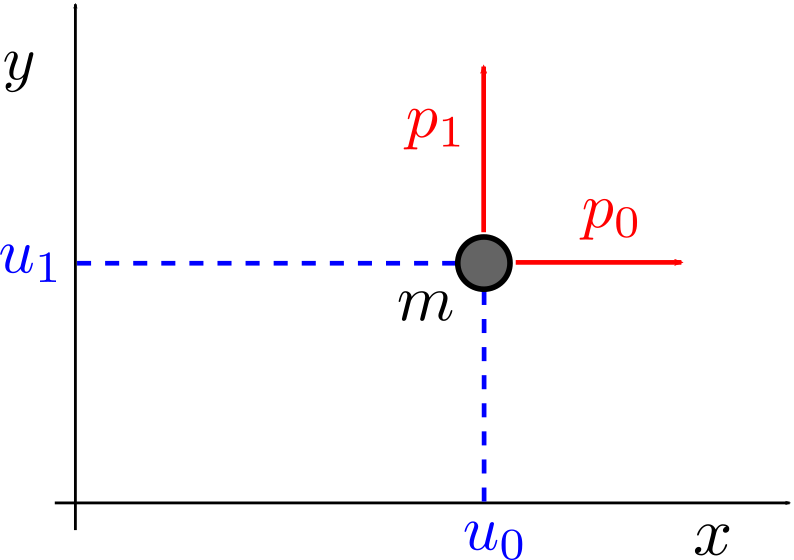
\includegraphics[width=0.4\textwidth]{figures/elements/mass-element}
\caption{Point mass element}
\label{fig:elements:point-mass}
\end{figure}

The equation of motion for this system can be written down directly by using Newton's second law of motion:

\begin{equation}
\underbrace{
\begin{bmatrix}
m & 0\\
0 & m
\end{bmatrix}
}_{\boldsymbol{M}}
\underbrace{
\begin{bmatrix}
\ddot{u}_0\\
\ddot{u}_1
\end{bmatrix}
}_{\boldsymbol{\ddot{u}}}
+
\underbrace{
\begin{bmatrix}
0\\
0
\end{bmatrix}
}_{\boldsymbol{q}(\boldsymbol{u},\,\dot{\boldsymbol{u}})}
=
\underbrace{
\begin{bmatrix}
p_0\\
p_1
\end{bmatrix}
}_{\boldsymbol{p}(t)}
\end{equation}

This immediately gives us the element's mass matrix, internal forces (which are zero) and external forces.
Because the internal forces are zero, the tangent stiffness matrix is zero as well:

\begin{equation}
\boldsymbol{K} = \frac{\partial \boldsymbol{q}}{\partial \boldsymbol{u}} =
\begin{bmatrix}
0 & 0\\
0 & 0
\end{bmatrix}.
\end{equation}

\newpage
\section{Bar Element}

A bar only transfers forces in longitudinal direction, it has no bending stiffness. Figure~\ref{fig:bar-element-1} shows a bar with an initial length of~$L$ that is subjected to a normal force~$N$ which causes it to elongate by~$\Delta L$.

\begin{figure}[h]
\centering
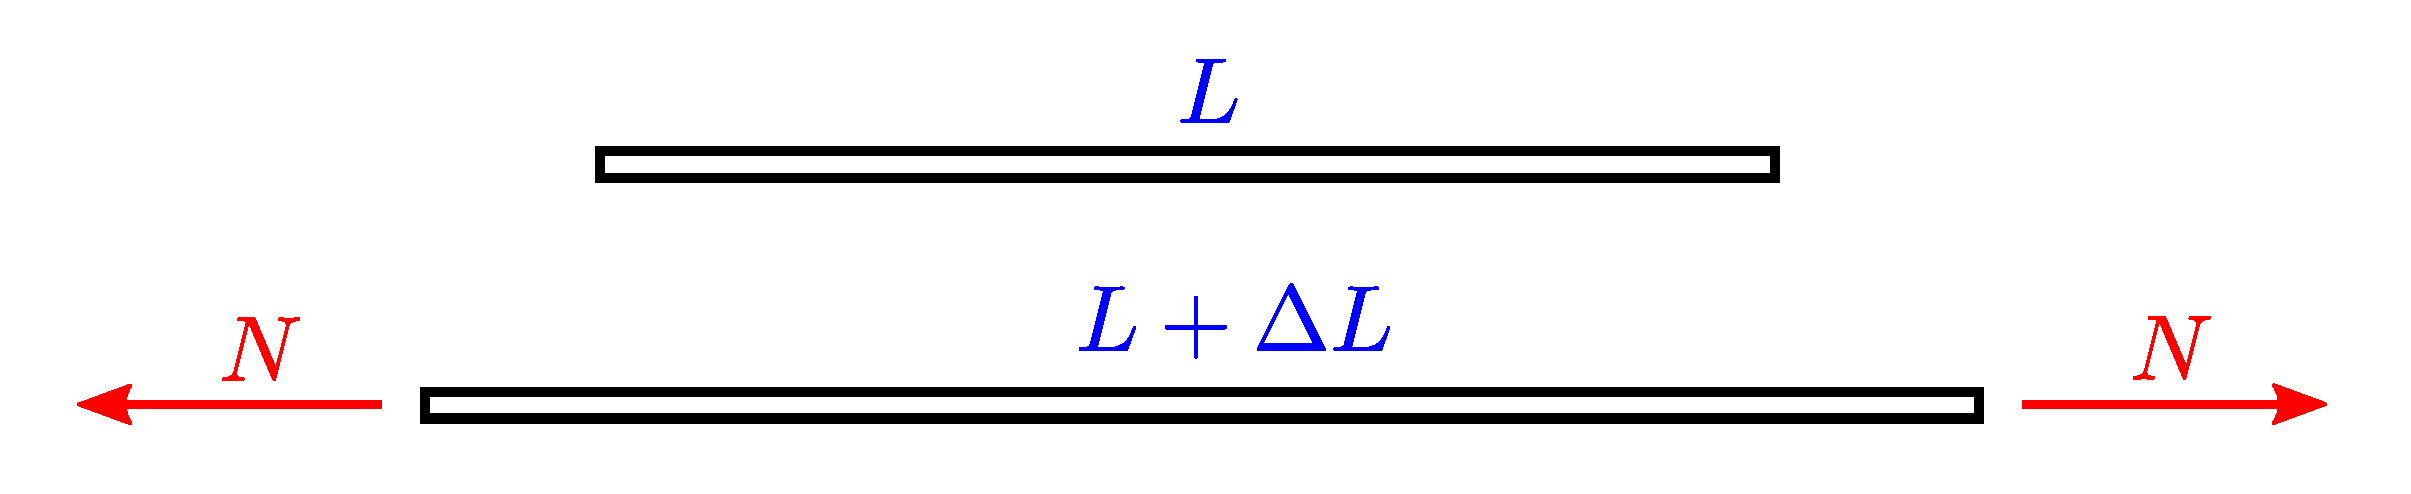
\includegraphics[width=0.75\textwidth]{figures/elements/bar-element-1}
\caption{Elongation of a bar under load}
\label{fig:bar-element-1}
\end{figure}

In order to simulate the damping properties of the string, a viscoelastic material model of the form

\begin{equation}
\sigma = E\,\varepsilon + \eta\,\dot{\varepsilon}
\end{equation}

is chosen. Here $E$ is the elastic modulus and $\eta$ the viscosity of the material. This model is called the Kelvin-Voigt model and combines linear elastic and linear viscous behaviour. The normal force in the bar given a constant cross section area $A$ is therefore

\begin{align}
N &= \sigma\,A \notag \\
&= EA\,\epsilon + \eta A\,\dot{\varepsilon} \notag \\
&= \frac{EA}{L}\,\Delta L + \frac{\eta A}{L}\,\Delta \dot{L}.\label{eq:bar-constitutive}
\end{align}

The product~$EA$ is also called the longitudinal stiffness. The bar is now placed between the two nodes A and B as shown in figure~\ref{fig:bar-element-2}. Its configuration is described by the nodal displacements~$\boldsymbol{u} = (u_0,\,u_1,\,u_2,\,u_3)^\mathsf{T}$.

\begin{figure}[h]
\centering
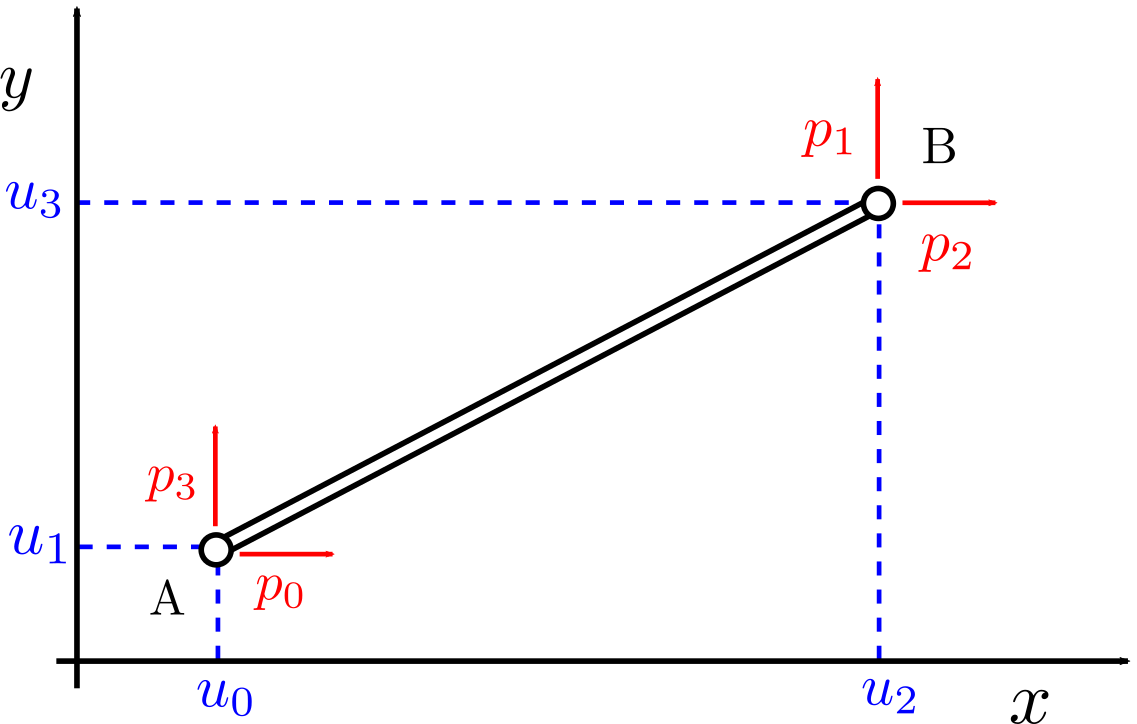
\includegraphics[width=0.6\textwidth]{figures/elements/bar-element-2}
\caption{Bar element}
\label{fig:bar-element-2}
\end{figure}

The position vectors of the two nodes are given by

\begin{equation}
\boldsymbol{r}_A =
\begin{bmatrix} u_0 \\ u_1 \end{bmatrix}, \quad
\boldsymbol{r}_B =
\begin{bmatrix} u_2 \\ u_3 \end{bmatrix}.\label{bar:node-positions}
\end{equation}

The mass of the element is assumed to be concentrated at the nodes, so that each of them is carrying half of the total mass.
This is called a lumped mass approach and will later lead to a constant, diagonal mass matrix.
For a bar with density~$\rho$ the mass of a node is therefore~$\frac{1}{2}\rho A L$. With this in mind we can write down Newton's second law of motion for each of the two nodes,
%
\begin{align}
\frac{\rho A L}{2}\,\ddot{\boldsymbol{r}}_A = \boldsymbol{q}_A + \boldsymbol{p}_A,\label{eq:bar-newton-1}\\
\frac{\rho A L}{2}\,\ddot{\boldsymbol{r}}_B = \boldsymbol{q}_B + \boldsymbol{p}_B.\label{eq:bar-newton-2}
\end{align}

Here,~$\boldsymbol{q}_A$,~$\boldsymbol{q}_B$ are the elastic forces that the bar exerts to the respective nodes and~$\boldsymbol{p}_A$,~$\boldsymbol{p}_B$ are the externally applied loads. The elastic forces can be obtained by multiplying the scalar normal force~$N$ in the bar~(\ref{eq:bar-constitutive}) with the tangent vector of the connecting line between the two nodes to account for the direction,
%
\begin{equation}
\boldsymbol{q}_A = N\,\frac{\boldsymbol{r}_B - \boldsymbol{r}_A}{|\boldsymbol{r}_B - \boldsymbol{r}_A|},\quad \boldsymbol{q}_B = -\boldsymbol{q}_A.\label{eq:bar-elastic}
\end{equation}

The elongation~$\Delta L$ can be calculated by subtracting the initial length of the element from its actual length,
%
\begin{align}
\Delta L &= |\boldsymbol{r}_B - \boldsymbol{r}_A| - L,\label{eq:bar-elongation} \\
\Delta \dot{L} &= \frac{d}{dt}\,|\boldsymbol{r}_B - \boldsymbol{r}_A| = \frac{\boldsymbol{r}_B - \boldsymbol{r}_A}{|\boldsymbol{r}_B - \boldsymbol{r}_A|}\,(\dot{\boldsymbol{r}}_B - \dot{\boldsymbol{r}}_A).\label{eq:bar-elongation-velocity}
\end{align}

Combining equations~(\ref{eq:bar-newton-1}),~(\ref{eq:bar-newton-2}) with~(\ref{eq:bar-elastic}),~(\ref{eq:bar-elongation}) and (\ref{eq:bar-elongation-velocity}) leads to the element's equation of motion,

\begin{equation}
\frac{\rho A L}{2}
\begin{bmatrix}
\ddot{\boldsymbol{r}}_A \\ \ddot{\boldsymbol{r}}_B
\end{bmatrix}
+
\frac{\eta A}{L}
\begin{bmatrix}
\dot{\boldsymbol{r}}_A - \dot{\boldsymbol{r}}_B \\ \dot{\boldsymbol{r}}_B - \dot{\boldsymbol{r}}_A
\end{bmatrix}
+
\frac{EA}{L}\left( 1 - \frac{L}{|\boldsymbol{r}_B - \boldsymbol{r}_A|} \right)
\begin{bmatrix}
\boldsymbol{r}_A - \boldsymbol{r}_B \\ \boldsymbol{r}_B - \boldsymbol{r}_A
\end{bmatrix}
=
\begin{bmatrix}
\boldsymbol{p}_A \\ \boldsymbol{p}_B
\end{bmatrix}.
\end{equation}

With~(\ref{bar:node-positions}) and the abbreviations $\Delta x = u_{2} - u_{0}$, $\Delta y = u_{3} - u_{1}$ this expands to

\begin{equation}
\underbrace{
\frac{\rho A L}{2}
\begin{bmatrix}
1\\
& 1\\
&& 1\\
&&& 1
\end{bmatrix}
}_{\boldsymbol{M}}
\underbrace{
\begin{bmatrix}
\ddot{u}_0\\
\ddot{u}_1\\
\ddot{u}_2\\
\ddot{u}_3
\end{bmatrix}
}_{\boldsymbol{\ddot{u}}}
+
\underbrace{
\frac{\eta A}{L}
\begin{bmatrix}
-\Delta \dot{x}\\
-\Delta \dot{y}\\
\ \ \Delta \dot{x}\\
\ \ \Delta \dot{y}
\end{bmatrix}
+
\frac{EA}{L}\left(1 - \frac{L}{\sqrt{\Delta x^2 + \Delta y^2}}\right)
\begin{bmatrix}
-\Delta x\\
-\Delta y\\
\ \ \Delta x\\
\ \ \Delta y
\end{bmatrix}
}_{\boldsymbol{q}(\boldsymbol{u},\,\dot{\boldsymbol{u}})}
=
\underbrace{
\begin{bmatrix}
p_0\\
p_1\\
p_2\\
p_3
\end{bmatrix}
}_{\boldsymbol{p}}.
\end{equation}

Note that the vector~$\boldsymbol{q}$ of internal forces depends on the displacements in a nonlinear way despite the bar itself being considered linear-elastic. The nonlinearity arises only from the geometry of the arbitrarily large nodal displacements. This is called geometric nonlinearity as opposed to material nonlinearity.

Deriving the internal forces with respect to $\boldsymbol{u}$ results in the tangent stiffness matrix
%
\begin{align*}
\boldsymbol{K} = \frac{\partial \boldsymbol{q}}{\partial \boldsymbol{u}} &=
\frac{EA}{L}\left(1 - \frac{L}{\sqrt{\Delta x^2 + \Delta y^2}}\right)
\begin{bmatrix}
1 & 0 & -1 & 0\\
0 & 1 & 0 & -1\\
-1 & 0 & 1 & 0\\
0 & -1 & 0 & 1
\end{bmatrix}\\
&+
\frac{EA}{(\sqrt{\Delta x^2 + \Delta y^2})^{3}}
\begin{bmatrix}
\Delta x^2 & \Delta x \Delta y & -\Delta x^2 & -\Delta x \Delta y\\
\Delta x \Delta y & \Delta y^2 & -\Delta x \Delta y & - \Delta y^2\\
-\Delta x^2 & -\Delta x \Delta y & \Delta x^2 & \Delta x \Delta y\\
-\Delta x \Delta y & -\Delta y^2 & \Delta x \Delta y & \Delta y^2
\end{bmatrix}.\\
\end{align*}

Similarly, deriving the internal forces with respect to $\dot{\boldsymbol{u}}$ results in the tangent damping matrix
%
\begin{align*}
\boldsymbol{D} = \frac{\partial \boldsymbol{q}}{\partial \dot{\boldsymbol{u}}} &=
\frac{\eta A}{L}
\begin{bmatrix}
1 & 0 & -1 & 0\\
0 & 1 & 0 & -1\\
-1 & 0 & 1 & 0\\
0 & -1 & 0 & 1
\end{bmatrix}.
\end{align*}

\newpage
\section{Beam Element}

The beam element will be developed in several steps.
First of all we will consider a standard linear Euler-Bernoulli element for small deformations.
Next we're going to see how laminated cross sections can be accounted for.
Finally, the linear beam element will be used as the base for a fully geometrically nonlinear element by means of a floating frame of reference approach.

\subsection{Linear Euler-Bernoulli Beam}

Consider the beam element shown in figure~\ref{fig:beam-linear}.
In the undeformed reference state it is aligned with the $x$-axis and has an initial length of~$L$. The deformed state of the element is described by the (small) longitudinal and transversal displacements~$v(x,t)$ and~$w(x,t)$, which are continuous functions of both time and the position along the $x$-axis.

\begin{figure}[h]
\centering
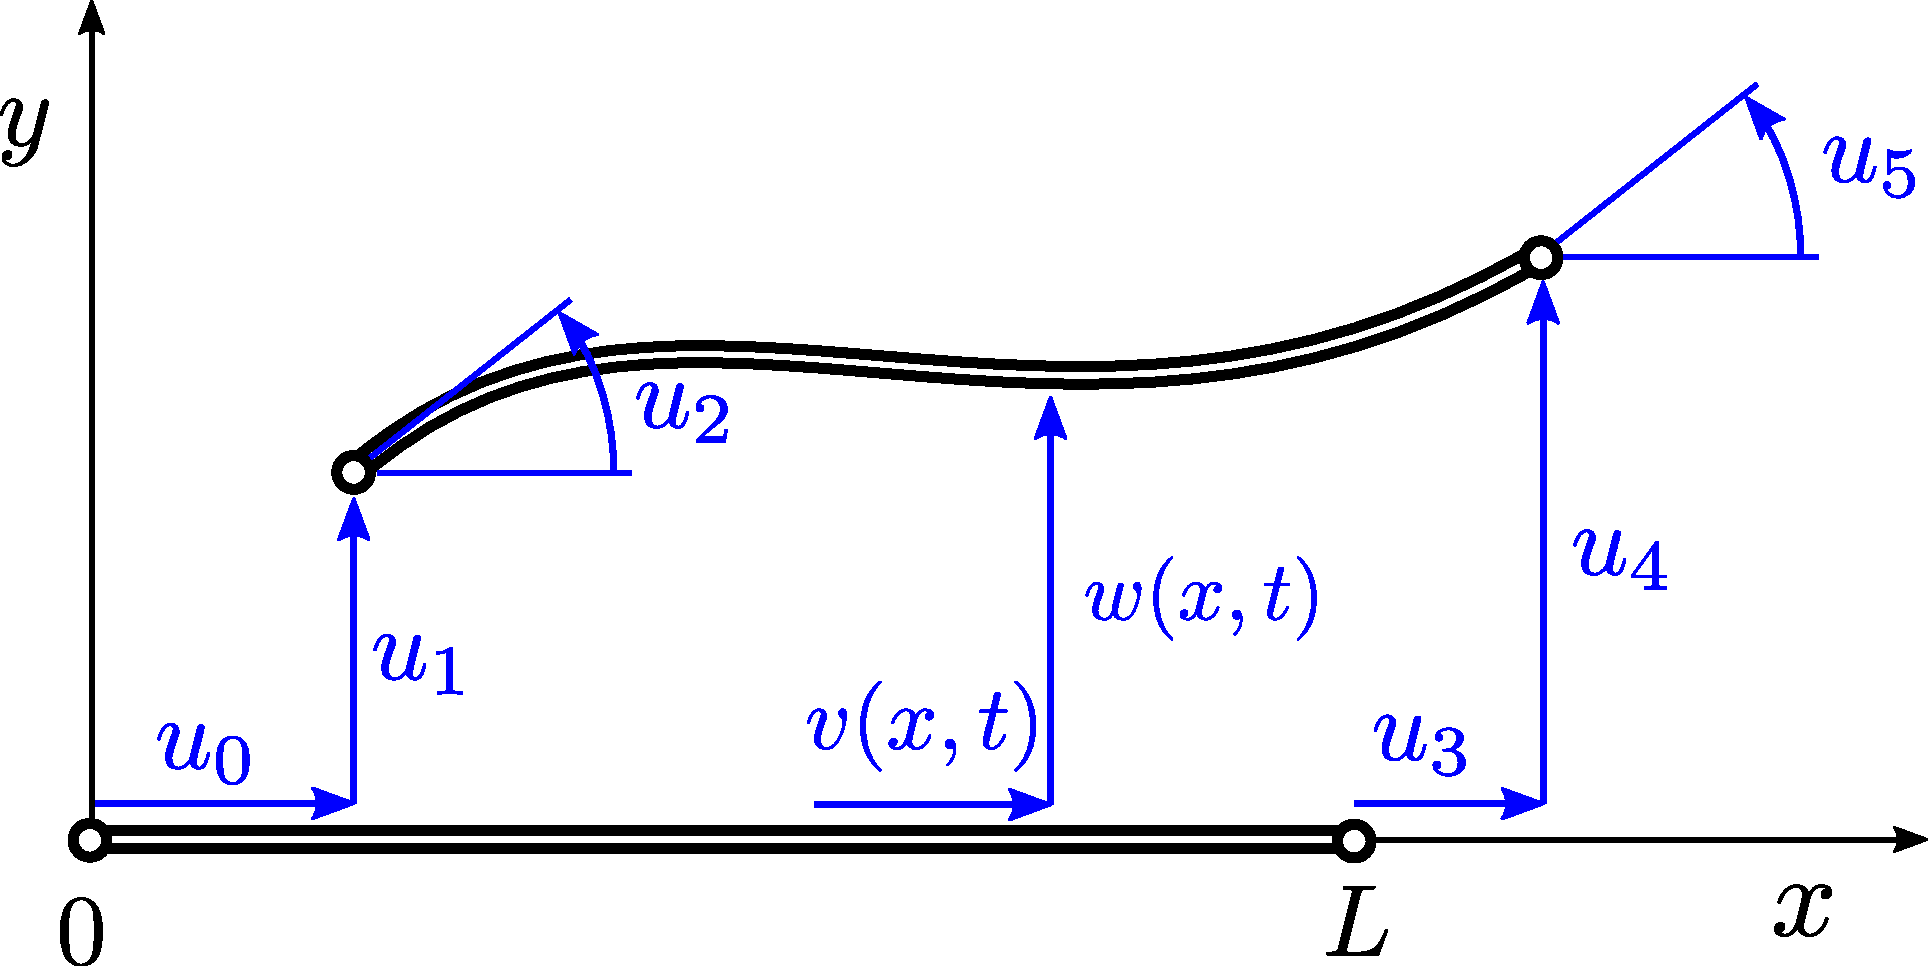
\includegraphics[width=0.7\textwidth]{figures/elements/beam-linear}
\caption{Beam element in reference and deformed configurations}
\label{fig:beam-linear}
\end{figure}

The finite element approach involves discretising this continuous displacement field by a finite number of degrees of freedom. This is achieved by choosing the nodal dispacements~$\boldsymbol{u}(t) = \begin{bmatrix}u_{0}(t),\ldots,\,u_{5}(t)\end{bmatrix}^\mathsf{T}$ as the degrees of freedom and interpolating~$v(x,t)$ and~$w(x,t)$ as

\begin{align}
v(x,t) &\approx \boldsymbol{V}(x)\,\boldsymbol{u}(t),\\
w(x,t) &\approx \boldsymbol{W}(x)\,\boldsymbol{u}(t),
\end{align}

with the shape functions~$\boldsymbol{V}(x)$ and~$\boldsymbol{W}(x)$.
As can be seen from figure~\ref{fig:beam-linear} the shape functions have to be chosen such that the following boundary conditions in regards to the nodal displacements are satisfied,

\begin{align}
v(0,t) &= u_{0}(t), & w(0,t) &= u_{1}(t), & w'(0,t) &= u_{2}(t),\notag\\
v(L,t) &= u_{3}(t), & w(L,t) &= u_{4}(t), & w'(L,t) &= u_{5}(t).\label{eq:elements:beam:boundary_conditions}
\end{align}

As the displacements were said to be small, the rotation angles of the nodes have been assumed to be equal to the derivative~$w'$ of the bending line here (small angle approximation).
Most frequently, for this standard type of beam element, cubic polynomials are used for~$\boldsymbol{W}(x)$ and a linear ones for~$\boldsymbol{V}(x)$. Coincidentally that is also the exact analytical solution for the static deformation of the beam. The free constants in those polynomials are determined by the boundary conditions~(\ref{eq:elements:beam:boundary_conditions}). The results are given by~\cite{bib:tm4} as

\begin{align}
\boldsymbol{W}(x) &=
\begin{bmatrix}
0\\
(1-\frac{x}{L})^2\,(1+2\,\frac{x}{L})\\
x\,(1-\frac{x}{L})^2\\
0\\
\frac{x^2}{L^2}\,(3-2\,\frac{x}{L})\\
-\frac{x^2}{L}\,(1-\frac{x}{L})
\end{bmatrix}^\mathrm{T},
&
\boldsymbol{V}(x) &=
\begin{bmatrix}
1-\frac{x}{L}\\
0\\
0\\
\frac{x}{L}\\
0\\
0
\end{bmatrix}^\mathrm{T}.
\end{align}

We now have a kinematic description of the beam element that has only a finite number of degrees of freedom. The vector of elastic forces $\boldsymbol{q}(\boldsymbol{u})$ for the system can be obtained by differentiating the system's total potential energy~\cite{bib:wiki-lagrange}, which in turn can be calculated by integrating the product of forces and deformations over the element length,

\begin{equation}
\boldsymbol{q}(\boldsymbol{u}) = \frac{\partial}{\partial \boldsymbol{u}}\,V(\boldsymbol{u}) = \frac{\partial}{\partial \boldsymbol{u}}\left(\frac{1}{2}\int_0^L
\begin{bmatrix}
N\\
M
\end{bmatrix}^\mathrm{T}
\begin{bmatrix}
\varepsilon\\
\kappa
\end{bmatrix}
\mathrm{d}x\right).\label{eq:beam-linear-energy-1}
\end{equation}

Here, $N$ and~$M$ are the normal force and the bending moment within the beam's cross sections, while $\varepsilon$ and $\kappa$ are the corresponding longitudinal strain and curvature of the beam's centerline. They are related to each other by the constitutive equation

\begin{equation}
\begin{bmatrix}
N\\
M
\end{bmatrix}
=
\begin{bmatrix}
C_{\varepsilon\varepsilon} & C_{\varepsilon\kappa}\\
C_{\varepsilon\kappa} & C_{\kappa\kappa}
\end{bmatrix}
\begin{bmatrix}
\varepsilon\\
\kappa
\end{bmatrix}.\label{eq:beam-constitutive}
\end{equation}

The constants $C_{\varepsilon\varepsilon}$, $C_{\kappa\kappa}$ and $C_{\varepsilon\kappa}$ are linear-elastic constants of the beam's cross section and will be determined later when we look at laminated beams. Combining the constitutive equation~(\ref{eq:beam-constitutive}) with~(\ref{eq:beam-linear-energy-1}), the elastic forces turn into

\begin{align}
\boldsymbol{q}(\boldsymbol{u}) &= \frac{\partial}{\partial \boldsymbol{u}}\left(\frac{1}{2}\int_0^L
\begin{bmatrix}
\varepsilon\\
\kappa
\end{bmatrix}^\mathrm{T}
\begin{bmatrix}
C_{\varepsilon\varepsilon} & C_{\varepsilon\kappa}\\
C_{\varepsilon\kappa} & C_{\kappa\kappa}
\end{bmatrix}
\begin{bmatrix}
\varepsilon\\
\kappa
\end{bmatrix}
\mathrm{d}x\right).\label{eq:elements:beam:total_energy_intermediate}
\end{align}

The strain~$\varepsilon$ and curvature~$\kappa$ for this beam can be calculated as

\begin{align}
\varepsilon(x,t) &= u'(x,t) = \boldsymbol{V}'(x)\,\boldsymbol{u}(t),\\
\kappa(x,t) &= w''(x,t) = \boldsymbol{W}''(x)\,\boldsymbol{u}(t).
\end{align}

Substituting these into equation~(\ref{eq:elements:beam:total_energy_intermediate}) finally leads to the following expression for the elastic forces,

\begin{align}
\boldsymbol{q}(\boldsymbol{u}) &= \frac{\partial}{\partial \boldsymbol{u}}\left(\frac{1}{2}\,\boldsymbol{u}^\mathrm{T}(t)
\underbrace{
\left(
\int_0^L
\begin{bmatrix}
\boldsymbol{V}'(x)\\
\boldsymbol{W}''(x)
\end{bmatrix}^\mathrm{T}
\begin{bmatrix}
C_{\varepsilon\varepsilon} & C_{\varepsilon\kappa}\\
C_{\varepsilon\kappa} & C_{\kappa\kappa}
\end{bmatrix}
\begin{bmatrix}
\boldsymbol{V}'(x)\\
\boldsymbol{W}''(x)
\end{bmatrix}
\mathrm{d}x
\right)
}_{\boldsymbol{C}}
\,\boldsymbol{u}(t)\right),\notag\\
&= \boldsymbol{C}\,\boldsymbol{u}(t).
\end{align}

The internal forces depend linearly on the displacements in a way that is determined by the stiffness matrix $\boldsymbol{C}$. Carrying out the integration yields

\begin{equation}
\boldsymbol{C} =
\begin{bmatrix}
\frac{1}{L}\,C_{\varepsilon\varepsilon} &
0 &
\frac{1}{L}\,C_{\varepsilon\kappa} &
-\frac{1}{L}\,C_{\varepsilon\varepsilon} &
0 &
-\frac{1}{L}\,C_{\varepsilon\kappa}\\ \\
0 &
\frac{12}{L^3}\,C_{\kappa\kappa} &
\frac{6}{L^2}\,C_{\kappa\kappa} &
0 &
-\frac{12}{L^3}\,C_{\kappa\kappa} &
\frac{6}{L^2}\,C_{\kappa\kappa}\\
\\
\frac{1}{L}\,C_{\varepsilon\kappa} &
\frac{6}{L^2}\,C_{\kappa\kappa} &
\frac{4}{L}\,C_{\kappa\kappa} &
-\frac{1}{L}\,C_{\varepsilon\kappa} &
-\frac{6}{L^2}\,C_{\kappa\kappa} &
\frac{2}{L}\,C_{\kappa\kappa}\\ \\
-\frac{1}{L}\,C_{\varepsilon\varepsilon} &
0 &
-\frac{1}{L}\,{C_{\varepsilon\kappa}} &
\frac{1}{L}\,C_{\varepsilon\varepsilon} &
0 &
\frac{1}{L}\,C_{\varepsilon\kappa}\\ \\
0 &
-\frac{12}{L^3}\,C_{\kappa\kappa} &
-\frac{6}{L^2}\,C_{\kappa\kappa} &
0 &
\frac{12}{L^3}\,C_{\kappa\kappa} &
-\frac{6}{L^2}\,C_{\kappa\kappa}\\ \\
-\frac{1}{L}\,C_{\varepsilon\kappa} &
\frac{6}{L^2}\,C_{\kappa\kappa} &
\frac{2}{L}\,C_{\kappa\kappa} &
\frac{1}{L}\,C_{\varepsilon\kappa} &
-\frac{6}{L^2}\,C_{\kappa\kappa} &
\frac{4}{L}\,C_{\kappa\kappa}
\end{bmatrix}.\label{eq:beam-linear-stiffness-matrix}
\end{equation}

The next step will be to determine the elastic constants $C_{\varepsilon\varepsilon}$, $C_{\kappa\kappa}$ and $C_{\varepsilon\kappa}$ for the kind of cross sections we're interested in.

\newpage
\subsection{Laminated Cross Sections}

The following derivations have been adapted from~\cite{bib:tm2} and~\cite{bib:wiki-sandwich}. Consider the laminated cross section shown in figure~\ref{fig:composite-sections-1}.
It is symmetric with respect to the~$y$-axis, bends/rotates around the~$z$-axis and consists of a number of rectangular layers. Each layer has its own density~$\rho_i$ and elastic modulus~$E_i$.
The geometry of the layers is given by their width~$w_i$, height~$h_i$ and center position~$y_i$.

\begin{figure}[h]
\centering
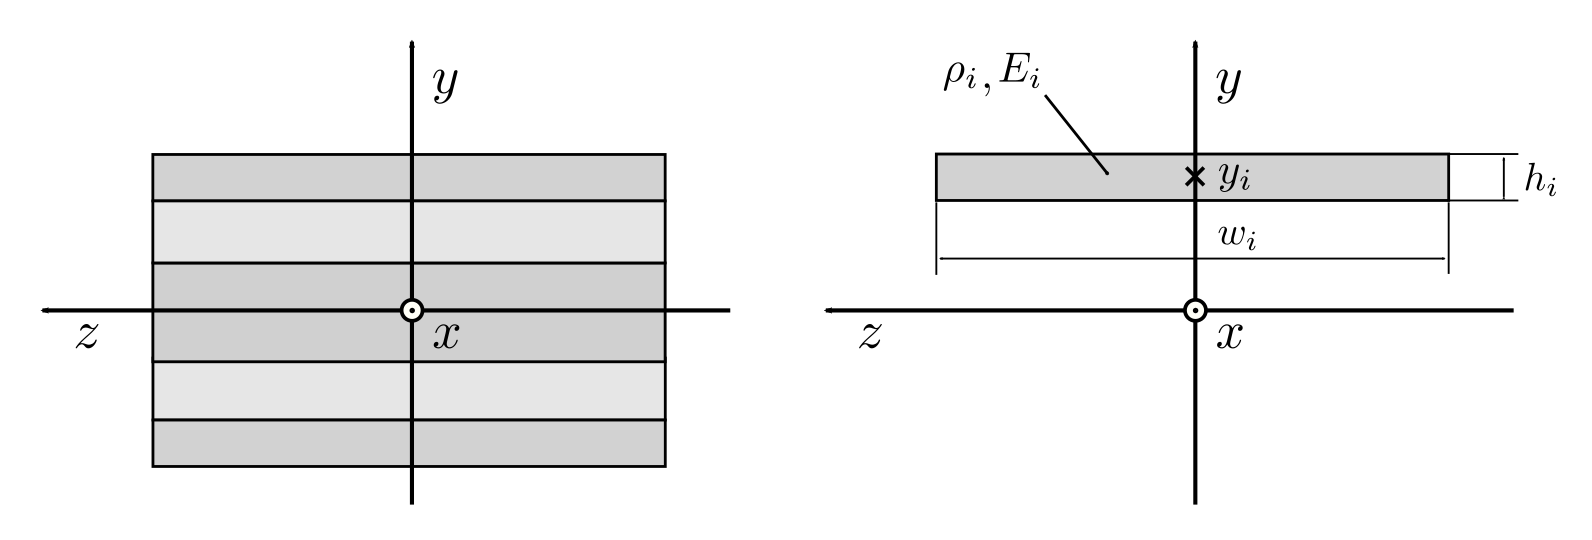
\includegraphics[width=0.9\textwidth]{figures/elements/composite-sections-1}
\caption{Composite cross section and single layer}
\label{fig:composite-sections-1}
\end{figure}

In Euler-Bernoulli beam theory the cross sections are assumed to stay flat and perpendicular to the beam axis during deformation.
We assume this to be true for our laminated cross section as well.
The distribution of longitudinal strain over the section is therefore given by the continuous function

\begin{equation}
\overline{\varepsilon}(y) = \varepsilon - \kappa\,y,
\end{equation}

where~$\varepsilon$ is the strain of the beam's centerline in $x$-direction and $\kappa$ its curvature around the $z$-axis.
The stress distribution however is not necessarily continuous, because each layer can have a different elastic modulus.
The stress within a layer is given by hooke's law as

\begin{equation}
\sigma_i(y) = E_i\cdot\overline{\varepsilon}(y),\quad y \in [y_i - \frac{h_i}{2},\,y_i + \frac{h_i}{2}].\label{eq:beam-stress-distribution}
\end{equation}

In order to determine the elastic constants in the constitutive equation~(\ref{eq:beam-constitutive}) we calculate the normal force~$N$ and bending moment~$M$ acting on the cross section by integrating the stresses~(\ref{eq:beam-stress-distribution}) over the section's area,

\begin{align}
N &= \int_A \sigma\,\mathrm{d}A = \sum_i\int_{A_i}\sigma_i\,\mathrm{d}A_i,\notag\\
&= \sum_i\int_{A_i}E_i\,\overline{\varepsilon}(y)\,\mathrm{d}A_i = \sum_i E_i \int_{A_i}(\varepsilon - \kappa\,y)\,\mathrm{d}A_i,\notag\\
&= \left(\sum_i E_i\int_{A_i}\mathrm{d}A_i\right)\varepsilon - \left(\sum_i E_i\int_{A_i}y\,\mathrm{d}A_i\right)\kappa,\notag\\
&=
\underbrace{
\left(\sum_i E_i\,A_i\right)
}_{C_{\varepsilon\varepsilon}}
\varepsilon
\underbrace{
- \left(\sum_i E_i\,A_i\,y_i\right)
}_{C_{\varepsilon\kappa}}
\kappa.\label{eq:elements:beam:constitutive_1}
\end{align}

The same can be done for the bending moment,

\begin{align}
M &= -\int_A y\,\sigma\,\mathrm{d}A = -\sum_i\int_{A_i}y\,\sigma_i\,\mathrm{d}A_i,\notag\\
&= -\sum_i\int_{A_i}y\,E_i\,(\varepsilon - \kappa\,y)\,\mathrm{d}A = -\sum_i\int_{A_i}(E_i\,\varepsilon\,y - E_i\,\kappa\,y^2)\,\mathrm{d}A,\notag\\
&= -\left(\sum_i E_i\int_{A_i}y\,dA_{i}\right)\varepsilon + \left(\sum_i E_i\int_{A_i}y^2\,dA_i\right)\kappa,\notag\\
&=
\underbrace{
-\left(\sum_i E_i\,A_i\,y_i\right)
}_{C_{\varepsilon\kappa}}
\varepsilon +
\underbrace{
\left(\sum_i E_i\,I_{i}\right)
}_{C_{\kappa\kappa}}
\kappa.\label{eq:elements:beam:constitutive_2}
\end{align}

The elastic constants describing the relationship between forces and deformation for the laminated cross section are therefore

\begin{align}
C_{\varepsilon\varepsilon} = \sum_i E_i\,A_i,\quad
C_{\kappa\kappa} = \sum_i E_i\,I_{i},\quad
C_{\varepsilon\kappa} = -\sum_i E_i\,A_i\,y_i.
\end{align}

In the case of the rectangular layers shown above, area~$A_i$ and second moment of inertia~$I_i$ evaluate to

\begin{align}
A_i &= w_i\,h_i,\\
I_i &= A_i\left(\frac{h_i^2}{12} + y_i^2\right).
\end{align}

Later we're also going to need the linear density (mass per unit length) of the laminated beam. It can be calculated by summing the the densities of the individual layers,

\begin{equation}
\overline{\rho A} = \sum_i \rho_i\,A_i.\label{eq:beam-linear-density}
\end{equation}

Pretty straightforward.

\newpage

\subsection{Floating Frame of Reference}

The floating frame of reference formulation is an easy way to construct a geometrically nonlinear finite element by reusing linear-elastic results.
The beam element is going to use a floating frame of reference approach based on~\cite{bib:beam_element_1} for the elastic forces, together with a lumped mass matrix according to~\cite{bib:beam_element_2}.
Key component is a floating frame of reference that is attached to the element and translates/rotates along with it.
The total motion of the element is then described as a superposition of two parts:

\begin{itemize}
\item The arbitrarily large, nonlinear rigid body motion (translation, rotation) of the reference frame
\item Small, linear-elastic deformations of the element with respect to its floating reference frame
\end{itemize}

Therefore the elastic deformation of the element can be treated as linear (because it's small), but on the other hand the element is still allowed to undergo arbitrarily large, nonlinear translations and rotations.
Note that we only assume the elastic deformations of the single elements to be small with respect to their frame of reference.
A structure composed of many such elements can still undergo large deformations as long as that assumption is valid. (And it can always be made valid by using enough elements.)

\begin{figure}[h]
\centering
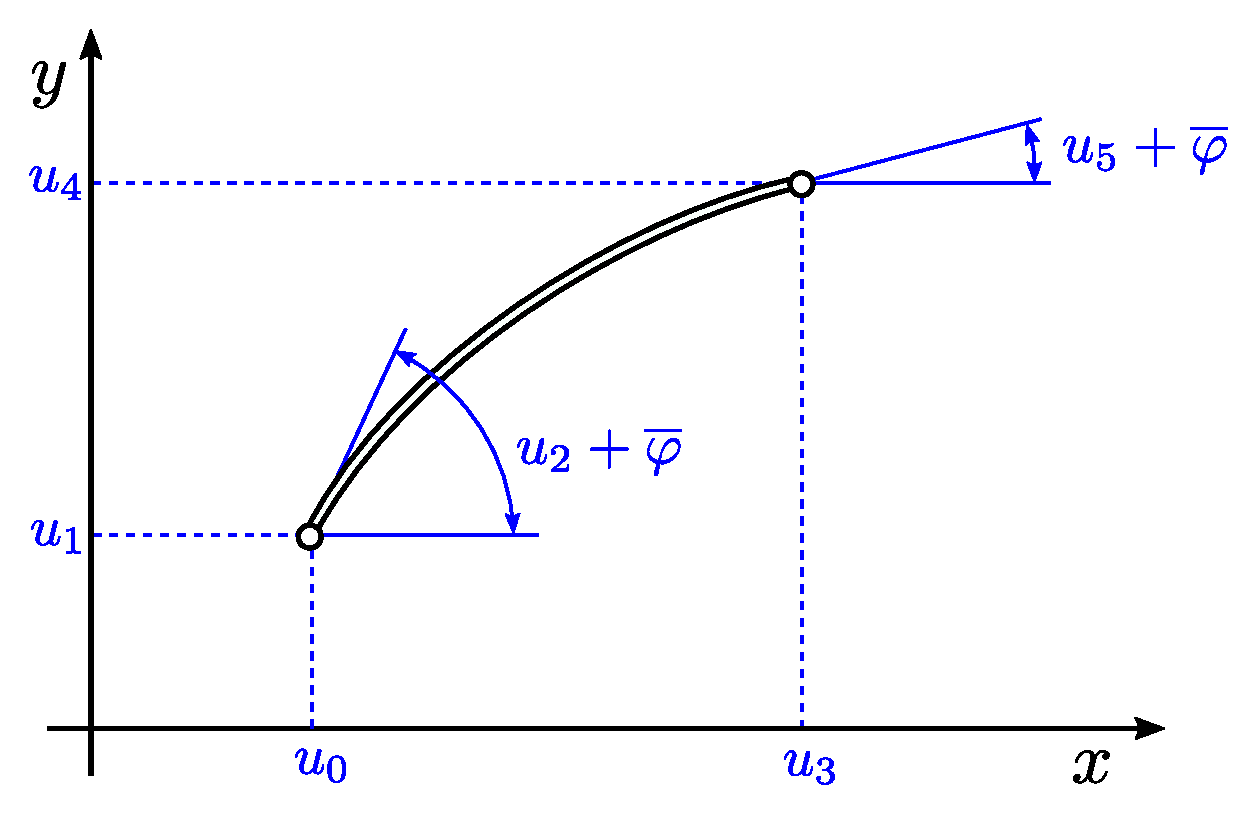
\includegraphics[width=0.6\textwidth]{figures/elements/beam-element-1}
\caption{Nodal displacements of the beam element}
\label{fig:beam-element-1}
\end{figure}

Let's apply this approach to the beam element shown in figure~\ref{fig:beam-element-1}. It has two nodes with the (arbitrarily large) nodal displacements~$\boldsymbol{u} = (u_0,\,\ldots,u_5)$ measured against the~$\{x,\,y\}$ coordinate system. The angle $\overline{\varphi}$ is a simple offset so that the rotation angles~$u_2$ and~$u_5$ don't necessarily have to correspond to the beam axis. This helps in practice when two adjacent elements share a node but are not tangential to each other.

We now introduce a floating frame of reference~$\{x',\,y'\}$ as shown in figure~\ref{fig:beam-element-2}. The $x'$-axis passes through both of the nodes (secant system) and the coordinate origin is placed at the left node. Within this reference system we now describe the elastic deformation with the three displacements~$\boldsymbol{e} = (e_0,\,e_1,\,e_2)^\mathsf{T}$, where~$e_0$ is the longitudinal extension of the beam and~$e_1$,~$e_2$ are the rotation angles of the nodes with respect to the~$x'$-axis.

\begin{figure}[h]
\centering
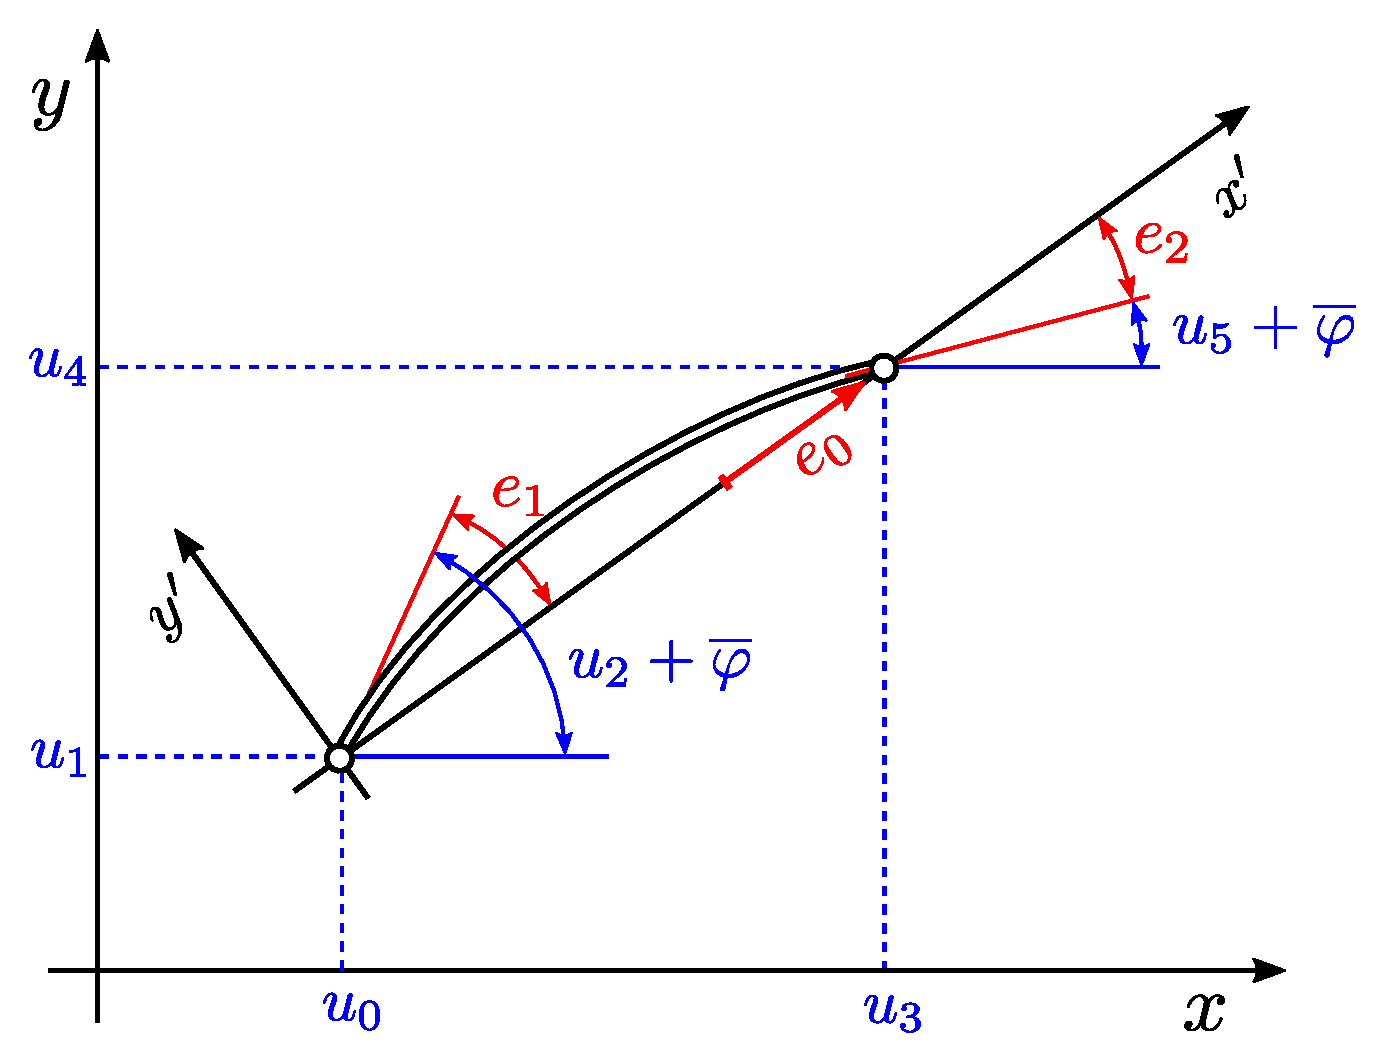
\includegraphics[width=0.6\textwidth]{figures/elements/beam-element-2}
\caption{Floating frame of reference and elastic deformations}
\label{fig:beam-element-2}
\end{figure}

Now obviously the elastic displacements~$\boldsymbol{e}$ depend on the overall displacements~$\boldsymbol{u}$ in some way, so the first thing we'll do is express this kinematic relationship. We introduce the auxiliary variables

\begin{align}
&\Delta x = u_3 - u_0,\\
&\Delta y = u_4 - u_1,\\
&\varphi = \mathrm{atan2} \left( \frac{\Delta y}{\Delta x} \right).
\end{align}

Here, $\varphi$ is the rotation angle of the floating reference frame. Using these abbreviations we can calculate the elastic deformations by using some elementary geometry.

\begin{align}
\intertext{Calculating $e_0$:}
&e_0 = \sqrt{\Delta x^2 + \Delta y^2} - L\\
\intertext{Calculating $e_1$:}
&\sin{(e_1)} = \sin{(u_2 + \overline{\varphi} - \varphi)} = \sin{(u_2)}\cos{(\overline{\varphi} - \varphi)} + \cos{(u_2)}\sin{(\overline{\varphi} - \varphi)}
\notag\\
&\cos{(e_1)} = \cos{(u_2 + \overline{\varphi} - \varphi)} = \cos{(u_2)}\cos{(\overline{\varphi} - \varphi)} - \sin{(u_2)}\sin{(\overline{\varphi} - \varphi)}\notag\\
&e_1 = \arctan{\left( \frac{\sin{(e_1)}}{\cos{(e_1)}} \right)}
\intertext{Calculating $e_2$:}
&\sin{(e_2)} = \sin{(u_5 + \overline{\varphi} - \varphi)} = \sin{(u_5)}\cos{(\overline{\varphi} - \varphi)} + \cos{(u_5)}\sin{(\overline{\varphi} - \varphi)}\notag\\
&\cos{(e_2)} = \cos{(u_5 + \overline{\varphi} - \varphi)} = \cos{(u_5)}\cos{(\overline{\varphi} - \varphi)} - \sin{(u_5)}\sin{(\overline{\varphi} - \varphi)}\notag\\
&e_2 = \arctan{\left( \frac{\sin{(e_2)}}{\cos{(e_2)}} \right)}
\intertext{Putting all those together, the elastic deformations can be written as}
&\boldsymbol{e}(\boldsymbol{u}) =
\begin{bmatrix}
\sqrt{\Delta x^2 + \Delta y^2} - L\\
\arctan{\left(\frac{\sin{(u_2)}\cos{(\overline{\varphi} - \varphi)}+\cos{(u_2)}\sin{(\overline{\varphi} - \varphi)}}{\cos{(u_2)}\cos{(\overline{\varphi} - \varphi)}-\sin{(u_2)}\sin{(\overline{\varphi} - \varphi)}}\right)}\\
\arctan{\left(\frac{\sin{(u_5)}\cos{(\overline{\varphi} - \varphi)}+\cos{(u_5)}\sin{(\overline{\varphi} - \varphi)}}{\cos{(u_5)}\cos{(\overline{\varphi} - \varphi)}-\sin{(u_5)}\sin{(\overline{\varphi} - \varphi)}}\right)}
\end{bmatrix}.\label{eq:beam-kinematics}
\end{align}

Having this out of the way, the vector of elastic forces~$\boldsymbol{q}(\boldsymbol{u})$ for the element will be obtained by differentiating the total potential energy~$V$ with respect to the displacements~$\boldsymbol{u}$,

\begin{equation}
\boldsymbol{q}(\boldsymbol{u}) = \frac{\partial V}{\partial \boldsymbol{u}}.\label{eq:beam-derivative}
\end{equation}

Now because we consider the beam as linear-elastic within its reference frame we can express its elastic energy as the quadratic expression

\begin{equation}
V = \boldsymbol{e}^\mathsf{T} \boldsymbol{C}\,\boldsymbol{e},
\end{equation}

where~$\boldsymbol{C}$ is the stiffness matrix of the beam. Its entries are a subset of the stiffness matrix ~(\ref{eq:beam-linear-stiffness-matrix}) that we derived earlier for the linear beam element,

\begin{equation}
\boldsymbol{C} =
\frac{1}{L}
\begin{bmatrix}
C_{\varepsilon\varepsilon} & -C_{\varepsilon\kappa} & C_{\varepsilon\kappa}\\
-C_{\varepsilon\kappa} & 4\,C_{\kappa\kappa} & 2\,C_{\kappa\kappa}\\
C_{\varepsilon\kappa} & 2\,C_{\kappa\kappa} & 4\,C_{\kappa\kappa}
\end{bmatrix}.
\end{equation}

Using this expression for the beam's energy, equation~(\ref{eq:beam-derivative}) becomes

\begin{align}
\boldsymbol{q}(\boldsymbol{u}) &= \frac{\partial V}{\partial \boldsymbol{u}} =  \frac{\partial V}{\partial \boldsymbol{e}}\,\frac{\partial \boldsymbol{e}}{\partial \boldsymbol{u}} = \left(\frac{\partial \boldsymbol{e}}{\partial \boldsymbol{u}}\right)^\mathsf{T}\boldsymbol{C}\,\boldsymbol{e}(\boldsymbol{u})\notag\\
&= \boldsymbol{J}(\boldsymbol{u})^\mathsf{T}\boldsymbol{C}\,\boldsymbol{e}(\boldsymbol{u}),
\end{align}

with the jacobian matrix $\boldsymbol{J}(\boldsymbol{u}) = \frac{\partial \boldsymbol{e}}{\partial \boldsymbol{u}}$. Differentiating~(\ref{eq:beam-kinematics}) gives us

\begin{align}
\boldsymbol{J}(\boldsymbol{u}) &= \frac{\partial \boldsymbol{e}}{\partial \boldsymbol{u}} =
\begin{bmatrix}
-J_{0} & -J_{1} & 0 & J_{0} & J_{1} & 0\\
-J_{3} & J_{2} & 1 & J_{3} & -J_{2} & 0\\
-J_{3} & J_{2} & 0 & J_{3} & -J_{2} & 1
\end{bmatrix},\\
\notag\\
J_{0} &= \frac{\Delta x}{\sqrt{\Delta x^2 + \Delta y^2}},\quad J_{1} = \frac{\Delta y}{\sqrt{\Delta x^2 + \Delta y^2}},\notag\\
\quad J_{2} &= \frac{\Delta x}{\Delta x^2 + \Delta y^2},\quad J_{3} = \frac{\Delta y}{\Delta x^2 + \Delta y^2}.
\end{align}

As always, the element's tangent stiffness matrix is obtained by differentiating the internal forces:

\begin{align}
\boldsymbol{K}(\boldsymbol{u}) &= \frac{\partial \boldsymbol{q}}{\partial \boldsymbol{u}} = \frac{\partial}{\partial \boldsymbol{u}}\left(\boldsymbol{J}^\mathsf{T}(\boldsymbol{u})\,\boldsymbol{C}\right)\boldsymbol{e}(\boldsymbol{u}) + \boldsymbol{J}^\mathsf{T}(\boldsymbol{u})\,\boldsymbol{C}\,\frac{\partial \boldsymbol{e}}{\partial \boldsymbol{u}}\notag\\
&= \left[\frac{\partial \boldsymbol{J}^\mathsf{T}(\boldsymbol{u})}{\partial u_{1}}\,\boldsymbol{C}\boldsymbol{e}(\boldsymbol{u}),\ldots \frac{\partial \boldsymbol{J}^\mathsf{T}(\boldsymbol{u})}{\partial u_{6}}\,\boldsymbol{C}\boldsymbol{e}(\boldsymbol{u})\right] + \boldsymbol{J}^\mathsf{T}(\boldsymbol{u})\,\boldsymbol{C}\,\boldsymbol{J}(\boldsymbol{u}).
\end{align}

The partial derivatives of the jacobian matrix~$\boldsymbol{J}$ are:

\begin{align}
\frac{\partial \boldsymbol{J}}{\partial u_0} &=
\begin{bmatrix}
-b_{0} & -b_{2} & 0 & b_{0} &  b_{2} & 0\\
-b_{5} &  b_{3} & 0 & b_{5} & -b_{3} & 0\\
-b_{5} &  b_{3} & 0 & b_{5} & -b_{3} & 0
\end{bmatrix},\quad
\frac{\partial \boldsymbol{J}}{\partial u_2} = 0,\quad
\frac{\partial \boldsymbol{J}}{\partial u_4} = -\frac{\partial \boldsymbol{J}}{\partial u_1},\notag\\
\frac{\partial \boldsymbol{J}}{\partial u_1} &=
\begin{bmatrix}
-b_{2} & -b_{1} & 0 & b_{2} &  b_{1} & 0\\
-b_{4} &  b_{5} & 0 & b_{4} & -b_{5} & 0\\
-b_{4} &  b_{5} & 0 & b_{4} & -b_{5} & 0
\end{bmatrix},\quad
\frac{\partial \boldsymbol{J}}{\partial u_3} = -\frac{\partial \boldsymbol{J}}{\partial u_0},\quad
\frac{\partial \boldsymbol{J}}{\partial u_5} = 0.
\end{align}

With the abbreviations

\begin{align}
a_{0} &= \frac{1}{(\Delta x^2 + \Delta y^2)^{\frac{1}{2}}},\quad
a_{1}  = \frac{1}{\Delta x^2 + \Delta y^2}\notag\\
a_{2} &= \frac{1}{(\Delta x^2 + \Delta y^2)^{\frac{3}{2}}},\quad
a_{3}  = \frac{1}{(\Delta x^2 + \Delta y^2)^{2}}\\
\notag\\
b_{0} &= a_{2}\Delta x^2 - a_{0},\quad b_{1} = a_{2}\Delta y^2 - a_{0},\quad b_{2} = a_{2}\Delta x\Delta y\notag\\
b_{3} &= 2a_{3}\Delta x^2 - a_{1},\quad b_{4} = 2a_{3}\Delta y^2 - a_{1},\quad b_{5} = 2a_{3}\Delta x\Delta y
\end{align}

The mass matrix is constructed by lumping the total mass and inertia of the element to the nodes, like before.
The total mass is~$\overline{\rho A}\,L$, using the linear density~(\ref{eq:beam-linear-density}) of the laminated cross sections.
Each translational degree of freedom therefore carries half of that mass. But the nodes also have a rotational degree of freedom each.
As it turns out, distributing the rotational inertia of a beam cannot be done in such a straightforward way.
There is simply no single "solution", only different approximations.
One possibility, according to~\cite{bib:beam_element_2}, is to use the mass matrix

\begin{equation}
\boldsymbol{M} = 
\overline{\rho A}\,L
\begin{bmatrix}
\frac{1}{2}\\
& \frac{1}{2}\\
&& \alpha L^2\\
&&& \frac{1}{2}\\
&&&& \frac{1}{2}\\
&&&&& \alpha L^2
\end{bmatrix},
\end{equation}

where~$\alpha \in\ ]0,\,\nicefrac{1}{50}]$ is a tunable parameter. Tests with the bow simulation suggest that the choice of~$\alpha$ barely has any influence on the results. Therefore the maximum value~$\alpha = \nicefrac{1}{50}$ has been chosen for numerical reasons.

\newpage
\section{Contact element}

The contact element is used to treat contact between a point and a surface. It uses a simple penalty approach: If the distance between the point and the surface is positive, there is no contact and nothing happens. But if the distance is negative, a contact force proportional to the penetration is applied that pushes the point outwards. By selecting a reasonably high contact stiffness the penetration can be kept small enough for all practical purposes.

\begin{figure}[h]
\centering
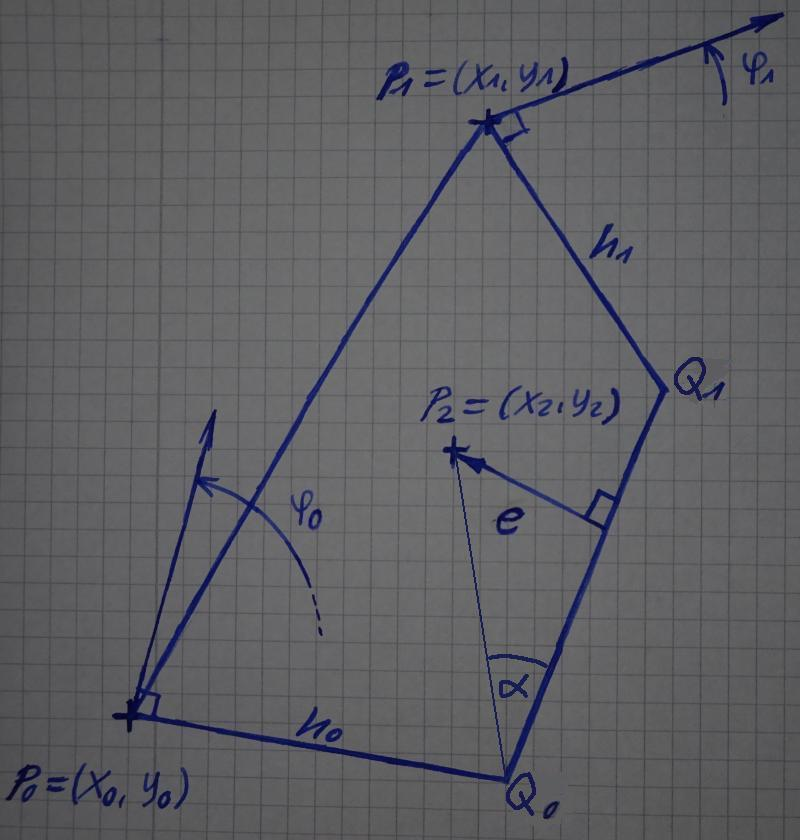
\includegraphics[width=0.5\textwidth]{figures/elements/contact_element_0}
\caption{Contact element}
%\label{fig:contact_element}
\end{figure}

\subsection{Contact Detection}

\textbf{Contact detection 1: Bounding box test}

\begin{align*}
x_{\rm{min}} &= \min\{x_0 - h_0,\:x_1 - h_1\}\\
y_{\rm{min}} &= \min\{y_0 - h_0,\:y_1 - h_1\}\\
x_{\rm{max}} &= \max\{x_0 + h_0,\:x_1 + h_1\}\\
y_{\rm{max}} &= \max\{y_0 + h_0,\:y_1 + h_1\}
\end{align*}

Necessary conditions for $P_2$ intersecting the segment:

\begin{align*}
x_{\rm{min}} \le x_{\rm{P2}} \le x_{\rm{max}}\\
y_{\rm{min}} \le y_{\rm{P2}} \le y_{\rm{max}}
\end{align*}

\textbf{Contact detection 2: Exact contact detection}

Coordinates of points $Q_0$ and $Q_1$:

\begin{equation*}
Q_0 = \begin{bmatrix}
x_{0} + h_{0}\sin(\varphi_{0}) \\
y_{0} - h_{0}\cos(\varphi_{0})
\end{bmatrix},\quad
Q_1 = \begin{bmatrix}
x_{1} + h_{1}\sin(\varphi_{1}) \\
y_{1} - h_{1}\cos(\varphi_{1})
\end{bmatrix}.
\end{equation*}

Define the four triangles

\begin{equation*}
T_{0} : \{ P_2, P_0, Q_0 \},\quad T_{1} : \{ P_2, P_1, P_0 \},\quad T_{2} : \{ P_2, Q_0, Q_1 \},\quad T_{3} : \{ P_2, Q_1, P_1 \}
\end{equation*}

$P_2$ lies inside the square if and only if all of the four triangles are oriented counter-clockwise. \textcolor{red}{[Citation needed]} % http://www.emanueleferonato.com/2012/03/09/algorithm-to-determine-if-a-point-is-inside-a-square-with-mathematics-no-hit-test-involved/
% https://en.wikipedia.org/wiki/Point_in_polygon

A triangle $\{A, B, C\}$ is oriented counter-clockwise if

\begin{align*}
&(B-A)\times(C-A) > 0,\\
\Leftrightarrow\quad &(x_B-x_A)(y_C-y_A)-(y_B-y_A)(x_C-x_A) > 0.
\end{align*}

\textbf{Contact detection 3: Penetration}

\begin{align*}
\sin(\alpha) &= \frac{e}{|P_2 - Q_0|} = \frac{(Q_1 - Q_0)\times(P_2 - Q_0)}{|Q_1 - Q_0||P_2 - Q_0|}\\
\\
\Leftrightarrow\:e &= \frac{(Q_1 - Q_0)\times(P_2 - Q_0)}{|Q_1 - Q_0|}\\
&= \frac{(x_{\rm{Q1}}-x_{\rm{Q0}})(y_{\rm{P2}}-y_{\rm{Q0}})-(y_{\rm{Q1}}-y_{\rm{Q0}})(x_{\rm{P2}}-x_{\rm{Q0}})}{\sqrt{(x_{\rm{Q1}}-x_{\rm{Q0}})^2+(y_{\rm{Q1}}-y_{\rm{Q0}})^2}}\\
&= \frac{a_1 a_4 - a_2 a_3}{\sqrt{a_1^2 + a_2^2}}
\intertext{With the abbreviations}
a_1 &= x_1 - x_0 - h_0 \sin(\varphi_0) + h_1 \sin(\varphi_1)\\
a_2 &= y_1 - y_0 + h_0 \cos(\varphi_0) - h_1 \cos(\varphi_1)\\
a_3 &= x_2 - x_0 - h_0 \sin(\varphi_0)\\
a_4 &= y_2 - y_0 + h_0 \cos(\varphi_0)
\end{align*}

\subsection{Contact Forces}

\textbf{Elastic forces}

The potential energy of the system can be determined as

\begin{align*}
V &= \int_{0}^{e}F(s)\,ds
\end{align*}

which yields the vector of elastic forces

\begin{align}
\boldsymbol{q}(\boldsymbol{u}) &= \frac{\partial V}{\partial \boldsymbol{u}} = \frac{\partial V}{\partial e}\frac{\partial e}{\partial \boldsymbol{u}} = F(e)\,\frac{\partial e}{\partial \boldsymbol{u}}.
\end{align}

Taking the derivatives:

\begin{align*}
\frac{\partial e}{\partial \boldsymbol{u}} &= \frac{\partial}{\partial \boldsymbol{u}}\left(\frac{a_1 a_4 - a_2 a_3}{\sqrt{a_1^2 + a_2^2}}\right)\\
&= \frac{\partial}{\partial \boldsymbol{u}}\left(\frac{1}{\sqrt{a_1^2 + a_2^2}}\right)\left(a_1 a_4 - a_2 a_3\right) + \frac{1}{\sqrt{a_1^2 + a_2^2}}\,\frac{\partial}{\partial \boldsymbol{u}}\left(a_1 a_4 - a_2 a_3\right)\\
&=
\underbrace{\frac{1}{\sqrt{a_1^2 + a_2^2}}}_{b_1} \underbrace{\left(a_4\frac{\partial a_1}{\partial \boldsymbol{u}} - a_3\frac{\partial a_2}{\partial \boldsymbol{u}} - a_2\frac{\partial a_3}{\partial \boldsymbol{u}} + a_1\frac{\partial a_4}{\partial \boldsymbol{u}}\right)}_{\boldsymbol{v}_1}
\underbrace{+\frac{a_2 a_3 - a_1 a_4}{(a_1^2 + a_2^2)^\frac{3}{2}}}_{b_2}
\underbrace{\left(a_1\frac{\partial a_1}{\partial \boldsymbol{u}} + a_2\frac{\partial a_2}{\partial \boldsymbol{u}}\right)}_{\boldsymbol{v}_2}\\
&= b_1\boldsymbol{v}_1 + b_2\boldsymbol{v}_2\\
\\
\frac{\partial a_1}{\partial \boldsymbol{u}} &=
\begin{bmatrix}
-1\\ 0\\ -h_0 \cos(\varphi_0)\\ 1\\ 0\\ h_1 \cos(\varphi_1)\\ 0\\ 0
\end{bmatrix},
\frac{\partial a_2}{\partial \boldsymbol{u}} =
\begin{bmatrix}
0\\ -1\\ -h_0 \sin(\varphi_0)\\ 0\\ 1\\ h_1 \sin(\varphi_1)\\ 0\\ 0
\end{bmatrix},
\frac{\partial a_3}{\partial \boldsymbol{u}} =
\begin{bmatrix}
-1\\ 0\\ -h_0 \cos(\varphi_0)\\ 0\\ 0\\ 0\\ 1\\ 0
\end{bmatrix},
\frac{\partial a_4}{\partial \boldsymbol{u}} =
\begin{bmatrix}
0\\ -1\\ -h_0 \sin(\varphi_0)\\ 0\\ 0\\ 0\\ 0\\ 1
\end{bmatrix}
\end{align*}

\textbf{Tangent stiffness matrix}

\begin{align*}
\boldsymbol{K}(\boldsymbol{u}) &= \frac{\partial \boldsymbol{q}}{\partial \boldsymbol{u}} = \frac{\partial F}{\partial \boldsymbol{u}}\,\left(\frac{\partial e}{\partial \boldsymbol{u}}\right)^{\rm{T}} + F(e)\,\frac{\partial^2 e}{\partial \boldsymbol{u}^2} = \frac{\partial F}{\partial e}\,\frac{\partial e}{\partial \boldsymbol{u}}\left(\frac{\partial e}{\partial \boldsymbol{u}}\right)^{\rm{T}} + F(e)\,\frac{\partial^2 e}{\partial \boldsymbol{u}^2}\\
\\
\frac{\partial^2 e}{\partial \boldsymbol{u}^2} &= \frac{\partial}{\partial \boldsymbol{u}}\left(b_1\boldsymbol{v}_1 + b_2\boldsymbol{v}_2\right) = \frac{\partial b_1}{\partial \boldsymbol{u}}\,\boldsymbol{v}_1^{\rm{T}} + \frac{\partial b_2}{\partial \boldsymbol{u}}\,\boldsymbol{v}_2^{\rm{T}} + b_1\,\frac{\partial \boldsymbol{v}_1}{\partial \boldsymbol{u}} + b_2\,\frac{\partial \boldsymbol{v}_2}{\partial \boldsymbol{u}}\\
\frac{\partial b_1}{\partial \boldsymbol{u}} &= -\frac{1}{\left(a_1^2 + a_2^2\right)^{\frac{3}{2}}}\left(a_1\,\frac{\partial a_1}{\partial \boldsymbol{u}} + a_2\,\frac{\partial a_2}{\partial \boldsymbol{u}}\right)\\
\frac{\partial b_2}{\partial \boldsymbol{u}} &= \frac{\sqrt{a_1^2 + a_2^2}}{a_1^6 + 3\,a_1^4\,a_2^2 + 3\,a_1^2\,a_2^4 + a_2^6}\bigg(\left(2\,a_1^2\,a_4 - a_2^2\,a_4 - 3\,a_1\,a_2\,a_3\right)\frac{\partial a_1}{\partial \boldsymbol{u}}\\
&+ \left(a_1^2\,a_3 - 2\,a_2^2\,a_3 + 3\,a_1\,a_2\,a_4\right)\frac{\partial a_2}{\partial \boldsymbol{u}} + \left(a_2^3 + a_1^2\,a_2\right)\frac{\partial a_3}{\partial \boldsymbol{u}} + \left(-a_1^3 - a_1\,a_2^2\right)\frac{\partial a_4}{\partial \boldsymbol{u}}\bigg)\\
\\
\frac{\partial \boldsymbol{v}_1}{\partial \boldsymbol{u}} &= \frac{\partial a_4}{\partial \boldsymbol{u}}\left(\frac{\partial a_1}{\partial \boldsymbol{u}}\right)^{\rm{T}} - \frac{\partial a_3}{\partial \boldsymbol{u}}\left(\frac{\partial a_2}{\partial \boldsymbol{u}}\right)^{\rm{T}} - \frac{\partial a_2}{\partial \boldsymbol{u}}\left(\frac{\partial a_3}{\partial \boldsymbol{u}}\right)^{\rm{T}} + \frac{\partial a_1}{\partial \boldsymbol{u}}\left(\frac{\partial a_4}{\partial \boldsymbol{u}}\right)^{\rm{T}}\\
&+ a_4\,\frac{\partial^2 a_1}{\partial \boldsymbol{u}^2} - a_3\,\frac{\partial^2 a_2}{\partial \boldsymbol{u}^2} - a_2\,\frac{\partial^2 a_3}{\partial \boldsymbol{u}^2} + a_1\,\frac{\partial^2 a_4}{\partial \boldsymbol{u}^2}\\
\frac{\partial \boldsymbol{v}_2}{\partial \boldsymbol{u}} &=  \frac{\partial a_1}{\partial \boldsymbol{u}}\left(\frac{\partial a_1}{\partial \boldsymbol{u}}\right)^{\rm{T}} + \frac{\partial a_2}{\partial \boldsymbol{u}}\left(\frac{\partial a_2}{\partial \boldsymbol{u}}\right)^{\rm{T}} + a_1\,\frac{\partial^2 a_1}{\partial \boldsymbol{u}^2} + a_2\,\frac{\partial^2 a_2}{\partial \boldsymbol{u}^2}
\end{align*}

Second derivatives:

\begin{equation*}
\begin{aligned}
\left(\frac{\partial^2 a_1}{\partial \boldsymbol{u}^2}\right)_{ij} &=
\begin{cases}
\:\:\:h_0\,\sin(\varphi_0) & \text{$ij = (3,3)$}\\
-h_1\,\sin(\varphi_1) & \text{$ij = (6,6)$}\\
\:\:\:0 & \text{otherwise}
\end{cases}\\
\left(\frac{\partial^2 a_3}{\partial \boldsymbol{u}^2}\right)_{ij} &=
\begin{cases}
\:\:\:h_0\,\sin(\varphi_0) & \text{$ij = (3,3)$}\\
\:\:\:0 & \text{otherwise}
\end{cases}\\
\end{aligned}
\qquad
\begin{aligned}
\left(\frac{\partial^2 a_2}{\partial \boldsymbol{u}^2}\right)_{ij} &=
\begin{cases}
-h_0\,\cos(\varphi_0) & \text{$ij = (3,3)$}\\
\:\:\:h_1\,\cos(\varphi_1) & \text{$ij = (6,6)$}\\
\:\:\:0 & \text{otherwise}
\end{cases}\\
\left(\frac{\partial^2 a_4}{\partial \boldsymbol{u}^2}\right)_{ij} &=
\begin{cases}
-h_0\,\cos(\varphi_0) & \text{$ij = (3,3)$}\\
\:\:\:0 & \text{otherwise}
\end{cases}
\end{aligned}
\end{equation*}

\subsection{Broadphase Algorithm}

\textcolor{red}{TODO}